\chapter{Dynamic Operations}
 \label{chap:dynamic}
 \section{Introduction}
	\hspace{10mm} The dynamic operations are add/delete operation on either query or data graph. The dynamic version is also having large applications. The dynamic processing will help to generate the isomorphic mappings without computing the whole answer again. This will give a great improvement in time. The dynamic changes are allowed with one condition that the query or graph will remain connected at any point of time. The dynamic queries are processed non-deterministic-ally meaning the order of execution of the dynamic queries is undefined. 
	\hspace{10mm} The dynamic operations and its difficulties are shown below.
	\begin{table}[H]
\centering
\begin{tabular}{|m{4cm}|m{4cm}|m{4cm}|m{4cm}|}
\hline
\textbf{}                                  & \textbf{Query Add Edge}                     & \textbf{Query Remove edge}                                 & \textbf{Query Unchanged} \\ \hline
\textbf{Data Add Edge}                                  & \textbf{Easy}                     & \textbf{Difficult}                                 & \textbf{Easy} \\ \hline
\textbf{Data Remove Edge}                                  & \textbf{Easy}                     & \textbf{Difficult}                                 & \textbf{Easy} \\ \hline
\textbf{Data Unchanged}                                  & \textbf{Easy}                     & \textbf{Difficult}                                 & \textbf{Static} \\ \hline
\end{tabular}
\caption{Dynamic Changes Difficulty Level}
%\label{tab:lit}
\end{table}
\section{Intermediate Answers}
	The intermediate answers will be saved so that dynamic answers can be processed faster.
	\begin{figure}[h]
 \centering
%\centering
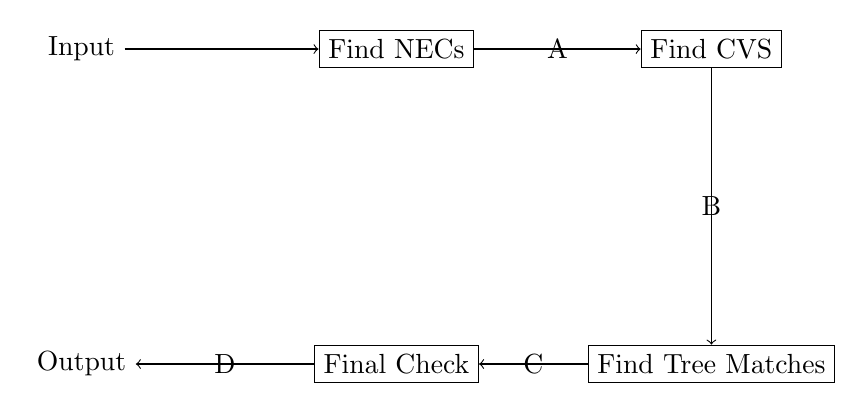
\begin{tikzpicture}[node distance=4cm]
\node[draw=none](6)[]{Input};
\node[rectangle,draw] (1)[right of=6]{Find NECs};
\node[rectangle,draw] (2)[right of=1]{Find CVS};
\node[rectangle,draw] (3)[below of=2]{Find Tree Matches};
\node[rectangle,draw] (4)[left of=3]{Final Check};
\node[draw=none](5)[left of =4]{Output};
\path[->]
	(6) edge node{} (1)
	(1) edge node{A} (2)
	(2) edge node{B} (3)
	(3) edge node{C} (4)
	(4) edge node {D} (5);
\end{tikzpicture}

 \caption{Intermediate Answers}
\end{figure}
	\hspace{10mm} A,B,C,D are the intermediate answer saved variables. A store the NECs of each vertec in query graph. B store CVS of each query vertex in data graph. C store the possible tree matches. D store the final exact graph maps.
\section{Adding Edge to Query Graph}
 \label{sec:aq}
	\hspace{10mm} It one of the easiest case because we need to check all the previous cases. The final answer will be a subset of previous answer.ie; Some of the matching will become invalid since the added edge may not be present. Only D changes.
	\hspace{10mm} Multiple queries can be done in parallel  by checking the existence of the added edges in all the previous answers. In parallel on all previous answers check the presence of added edges.
\section{Deleting Edge from Data Graph}
 \label{sec:dd}
	\hspace{10mm} It is also easy because the final answer is subset of previous answer.Multiple Queries can be processed similiar to the previous case.Only D changes.
	\hspace{10mm} Even if we needed to 
\section{Deleting Edge from Query Graph}
 \label{sec:dq}
	\hspace{10mm} This is a difficult case since we need to find the mappings that are going to be added. This case is divided into two parts.
\subsection{Deleting a non-tree edge}	
	\hspace{10mm} The tree inside the query graph remains unchanged. So the tree matches are correct. We need to go through all the tree matching(C) and check for possible additions of maps to final answer. So saving the intermediate answer C helps in finding the solution faster.
\subsection{Deleting a tree edge}	
	\hspace{10mm} Since the tree is changed here the CVS of vertices may change.So rather than calculating all the CVS there is a more efficient way. If a edge u-v in the tree is deleted and u is parent of v in tree. All the nodes in the path from u to root(parent,grand-parent,.. of u) should recalculate the CVS.
	 \hspace{10mm} When multiple queries are given the deletion may be from different parts of the tree. But each node should be processed once. 
\begin{algorithm}[H]
\caption{Dynamic tree edge deletion of thread t}
\textbf{Input}: Data Graph $D$,Query Graph $Q$,Delete u-v(u is parent of v).\\
\textbf{Output}: CVS updates.\\
\begin{algorithmic}
 \item \begin{enumerate}
 \item w=v
\item for each parent of w(till root)
 \begin{enumerate}
\item mark w for t
\end{enumerate}
\item for each parent of w(till root)
 \begin{enumerate}
\item if mark at w is t, acquire lock for w
\end{enumerate}
\item for each parent of w(till root)
\begin{enumerate}
\item if mark at w is t and able to acquire locks for all childs of w 
\item Recompute NEC of w
\item if not a previously computed NEC then
\item  \hspace{10mm}C(w)=$FindCandidates$(w,D) update
\item Release all locks
\end{enumerate}
\end{enumerate}
\end{algorithmic}
\end{algorithm}
	\hspace{10mm} The above algorithm marks all the parent nodes from a particular deleted edge. This marking helps to make sure only one thread process one node. The processing will be done such a way that no parent nodes are processed if any  child of the parent is unprocessed. So the processing order will be leaf to root. This will change the values inside A and so as B.
\section{Adding Edge in Data Graph}
 \label{sec:ad}
	\hspace{10mm} This will also add entries into B. But A will not be changed since no edges in query graph is changed. 
	\begin{algorithm}[H]
\caption{Dynamic data edge addition of thread t}
\textbf{Input}: Data Graph $D$,Query Graph $Q$,Delete u-v(u is parent of v).\\
\textbf{Output}: CVS updates.\\
\begin{algorithmic}
 \item \begin{enumerate}
 \item w=v (for u also)
\item for each child of w(till $|Q|$ length)
\begin{enumerate}
\item if acquire locks for all childs of w 
\item foreach NEC's x
\item C(x)=$FindCandidates$(x,D) update
\item Release all locks
\end{enumerate}
\end{enumerate}
\end{algorithmic}
\end{algorithm}
\hspace{10mm} This algorithm moves to  $|Q|$ length from both u and v in a BFS fashion. At each Data node it is checked whether it can be added to CVS of any of the NECs. When there is an overlap of regions of different thread locks are used to synchronize them. Since the Data graph is huge and  query graph is small and so the possibility of two edge deletion happening near( edge length  $< ~|Q|$ ) is small, the number of locks waits will be minimal.
\subsection{Parallel Execution}
\hspace{10mm} All the four quires can be processed in parallel since they are operating on different data. \ref{sec:aq} and \ref{sec:dd} are processing on D while \ref{sec:dq} and \ref{sec:ad} are processing on A and B. So it is safe to run them parallel. Parallel adding to A and B doesn't make the answer inconsistent. It will add a vertex into the CVS which  will be removed when exact matching is performed in the end.
\subsection{Inferences}
	\hspace{10mm} So a $Find Tree$ match algorithm should be done at each stage of the output to get the new possiblities. But this stage is the costliest of all the four steps. Even one vertex is added to any two CVS, this will cause to recompute most of the permutations and combinations again. So there is no computational advantage by dynamic processing. Running a subgraph isomorphism solution after applying all edge updates becomes equally fast as the dynamic version. 
